%coding:utf-8

%----------------------------------------
%FOSAPHY, a LaTeX-Code for a summary of linear systems and regulation
%Copyright (C) 2014, Mario Felder, Michael Fallegger

%This program is free software; you can redistribute it and/or
%modify it under the terms of the GNU General Public License
%as published by the Free Software Foundation; either version 2
%of the License, or (at your option) any later version.

%This program is distributed in the hope that it will be useful,
%but WITHOUT ANY WARRANTY; without even the implied warranty of
%MERCHANTABILITY or FITNESS FOR A PARTICULAR PURPOSE.  See the
%GNU General Public License for more details.
%----------------------------------------
\newpage
\section{Systeme}
\begin{center}
	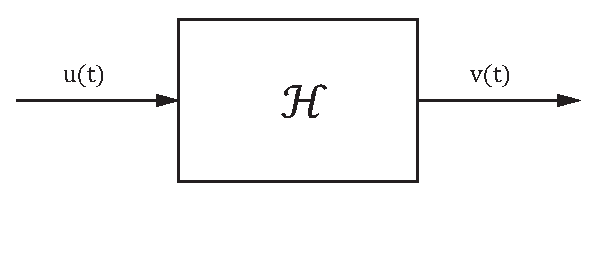
\includegraphics[scale = 0.5]{images/ss_system.eps}
\end{center}
Ein System ist eine Zuordnungsvorschrift, die eine Funktion $u(t)$ (Eingangssignal) in eine andere Funktion $v(t)$ (Ausganssignal) überführt.
\[
	\sysH{u(t)} = v(t)
\]

\subsection{Eigenschaften}
\subsubsection{Linear}
Ein System ist linear, wenn die folgenden beiden Eigenschaften gelten:
\begin{itemize}
	\item Das System antwortet auf ein amplifiziertes Eingangssignal mit der Verstärkung des Ausgangssignals um den gleichen Faktor:
	\[
		\sysH{A \cdot u(t)}= A \cdot \sysH{u(t)} = A \cdot v(t)
	\]
	\begin{footnotesize}
		für jedes Eingangssignal $u(t)$ und jede Konstante $A \in \mathbb{R}$\\
	\end{footnotesize}
	\item Das Syastem antwortet auf eine Überlagerung zweier Signale mit der Überlagerung der beiden Ausgangssignale
	\[
		\sysH{u_1(t) + u_2(t)} = \sysH{u_1(t)} + \sysH{u_2(t)} = v_1(t) + v_2(t)
	\]
	\begin{footnotesize}
		für zwei beliebige Eingangssignale $u_1(t),u_2(t)$.\\\\
	\end{footnotesize}
\end{itemize}
Zusammengefasst:
\[
	\sysH{A_1 \cdot u_1(t) + A_2 \cdot u_2(t)} = A_1 \cdot v_1(t) + A_2 \cdot v_2(t)
\]

\subsubsection{Zeitinvariant}
Ein System ist zeitinvariant, wenn es auf ein Signal immer gleich regiert, egal zu welcher Zeit man das System mit einem Signal stimuliert:
\[
	\sysH{u(t-t_0)} = v(t-t_0)
\]